\begin{exercise}
      {ID-20aedaf3992ebc1b6ba8673186751504895c3c48}
      {Radius}
  \ifproblem\problem
    Berechne den Radius des grauen Kreises in Abhängigkeit von $a$.
    \begin{center}
      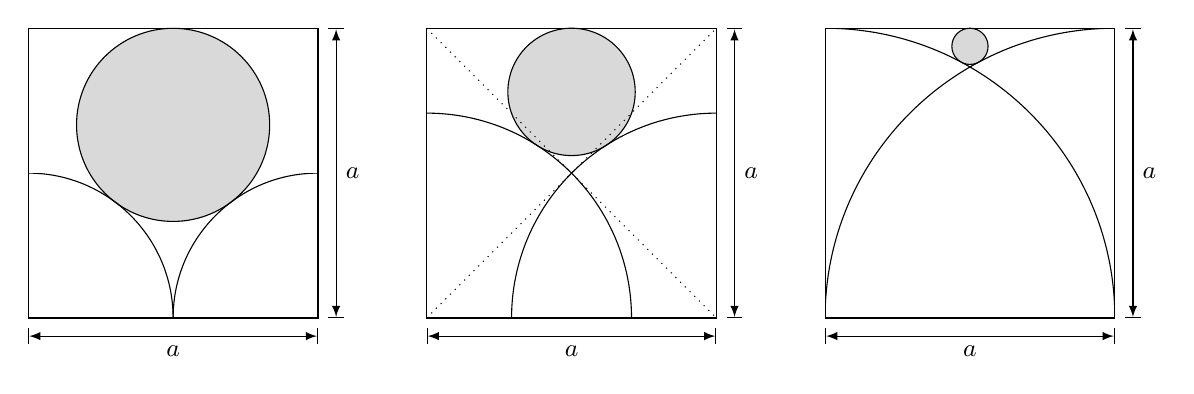
\begin{tikzpicture}[scale=0.92]
        % Figur 1
        \begin{scope}
          % Kreisflaeche
          \fill[fill=black!15!white] (2, 2.666) circle (1.333);
          % Quadrat
          \draw (0, 0) rectangle (4, 4);
          % Kreis
          \draw (2, 2.666) circle (1.333);
          % Viertelkreise
          \begin{scope}
            \clip (0, 0) rectangle (4, 2);
            \draw (0, 0) circle (2);
            \draw (4, 0) circle (2);
          \end{scope}
          % Bezeichnung
          \draw[|<->|, >=latex, shift={(0, -0.25)}] (0, 0) -- node[below] {{\small$a$}} (4, 0);
          \draw[|<->|, >=latex, shift={(0.25, 0)}] (4, 0) -- node[right] {{\small$a$}} (4, 4);
        \end{scope}
        % Figur 2
        \begin{scope}[xshift=5.5cm]
          % Kreisflaeche
          \fill[fill=black!15!white] (2, 3.121) circle (0.879);
          % Quadrat
          \draw (0, 0) rectangle (4, 4);
          % Diagonalen
          \draw[style=dotted] (0, 0) -- (4, 4);
          \draw[style=dotted] (0, 4) -- (4, 0);
          % Kreis
          \draw (2, 3.121) circle (0.879);
          % Kreise
          \begin{scope}
            \clip (0, 0) rectangle (4, 4);
            \draw (0, 0) circle (2.828);
            \draw (4, 0) circle (2.828);
          \end{scope}
          % Bezeichnung
          \draw[|<->|, >=latex, shift={(0, -0.25)}] (0, 0) -- node[below] {{\small$a$}} (4, 0);
          \draw[|<->|, >=latex, shift={(0.25, 0)}] (4, 0) -- node[right] {{\small$a$}} (4, 4);
        \end{scope}
        % Figur 3
        \begin{scope}[xshift=11cm]
          % Kreisflaeche
          \fill[fill=black!15!white] (2, 3.75) circle (0.25);
          % Quadrat
          \draw (0, 0) rectangle (4, 4);
          % Kreis
          \draw (2, 3.75) circle (0.25);
          % Kreise
          \begin{scope}
            \clip (0, 0) rectangle (4, 4);
            \draw (0, 0) circle (4);
            \draw (4, 0) circle (4);
          \end{scope}
          % Bezeichnung
          \draw[|<->|, >=latex, shift={(0, -0.25)}] (0, 0) -- node[below] {{\small$a$}} (4, 0);
          \draw[|<->|, >=latex, shift={(0.25, 0)}] (4, 0) -- node[right] {{\small$a$}} (4, 4);
        \end{scope}
      \end{tikzpicture}
    \end{center}
  \fi
  %\ifoutline\outline
  %\fi
  %\ifoutcome\outcome
  %\fi
\end{exercise}
